\chapter{绪论}{Introduction}
\section{概述}{Introduction}
\dots\\
\dots\\
\dots\\

\dots\\
\dots\\
\dots\\

\subsection{研究目标}
描述旋流-静态微泡浮选柱的旋流场结构,分析旋流场特征及其影响;
借助流体力学软件对柱体的内部流场进行模拟并分析其流场速度分布规律,
研究循环矿浆量及给矿量等因素对流场的影响;通过对旋流场内的颗粒受力分析,
建立基于旋流的颗粒动力学方程;系统揭示旋流分选作用,并进行相关动力学分析 \dots 

\subsection{研究方法}
流场模拟及分选机理研究,见下表\ref{tab:particle-size-distribution-results}。\\ 

\begin{table}
    \linespread{1.5}
    \zihao{5}
    \centering
    \caption{筛分粒度组成}{Particle size distribution results}
    \label{tab:particle-size-distribution-results}
    \begin{tabular}{ccccc}
    \bottomrule
    粒级,mm    & 产率,% & 灰分,% & 累计产率,% & 累计灰分,% \\ \hline
    >0.5     & 3.80 & 7.38 & 3.80   & 7.38   \\
    0.5~0.25 & 4.55 & 4.56 & 8.35   & 5.84   \\
    0.5~0.25 & 4.55 & 4.56 & 8.35   & 5.84   \\
    0.5~0.25 & 4.55 & 4.56 & 8.35   & 5.84   \\
    0.5~0.25 & 4.55 & 4.56 & 8.35   & 5.84   \\
    合计       & 4.55 & 4.56 & 8.35   & 5.84   \\ \bottomrule
    \end{tabular}
\end{table}


\begin{figure}
    \centering
    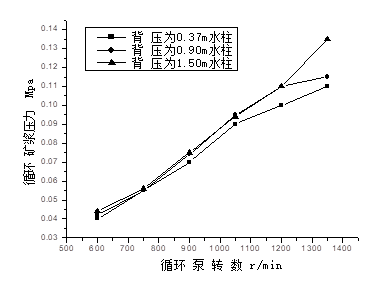
\includegraphics[]{figures/example.png}
    \caption{循环矿浆压力与柱体背压的关系}{Relationship between the pressure of circulating pulp and the back pressure}
    \label{circulating-pulp-and-the-backpressure-relationship} % label 用来在文中索引
\end{figure}
